\chapter{Authentication and authorization}\label{ch:authentication-and-authorization}


\section{Motivation}\label{sec:motivation}
In this section we describe the processes of Authentication and Authorization in the system.
It is worth to remember the meaning of Authentication and Authorization definitions.
Authentication -- is the process of ascertaining that somebody really is who they claim to be [\cite{burrows1989logic}].
Authorization refers to rules that determine who is allowed to do what [\cite{fagin1978authorization}].
For example, Adam may be authorized to create and delete databases, while Eve is only authorized to read.
The two concepts are completely orthogonal and independent, but both are central to security design, and the
failure to get either one correct opens up the avenue to compromise.
In terms of web apps, very crudely speaking, authentication is when you check login credentials to see if you recognize
a user as logged in, and authorization is when you look up in your access control whether you allow the user to view,
edit, delete or create content.
Currently, there are two widely-known authentication methods, that are cookie authentication and JWT (JSON Web Token)
authentication.
We discuss JWTs in next section.


\section{JWT Tokens}\label{sec:jwt-tokens}
JSON Web Token (JWT) is an open standard (RFC 7519) that defines a compact and self-contained way for securely
transmitting information between parties as a JSON object [\cite{jones2015json}].
This information can be verified and trusted because it is digitally signed.
JWTs can be signed using a secret (with the HMAC algorithm [\cite{wang2004hmac}]) or a public/private key pair using RSA or ECDSA\@.
Although JWTs can be encrypted to also provide secrecy between parties, we will focus on signed tokens.
Signed tokens can verify the integrity of the claims contained within it, while encrypted tokens hide those claims from
other parties.
When tokens are signed using public/private key pairs, the signature also certifies that only the party holding the
private key is the one that signed it.
In its compact form, JSON Web Tokens consist of three parts separated by dots, which are:
\begin{itemize}
    \item Header -- typically consists of two parts: the type of the token, which is JWT, and the signing algorithm
    being used, such as HMAC SHA256 or RSA\@.
    \item Payload -- The second part of the token is the payload, which contains the claims.
    Claims are statements about an entity (typically, the user) and additional data.
    There are three types of claims: registered, public, and private claims.
    \item Signature -- To create the signature part you have to take the encoded header, the encoded payload, a secret,
    the algorithm specified in the header, and sign that.
\end{itemize}
Therefore, a JWT typically looks like \texttt{xxxxx.yyyyy.zzzzz}.
Then, this JSON is Base64Url encoded to form the first part of the JWT\@.

As to the projects concerns, we should handle multiple client applications, e.g desktop,
web, mobile etc.
Therefore, cookie authorization doesn't fit for the project, however the JWT one surely passes.


\section{JWT Authentication}\label{sec:jwt-authentication}
Authentication (from the Greek [authentikos] - real, genuine;
by [authentes] - author) - it is process which verify user credentials, for instance login and password.
User authentication by comparing the login and password entered by him with the data saved in the database.
Authorization - it is process which check of the user's rights to access certain resources.

For example, after authentication the user Bob gets the right to access and get from resource
https://resource.com some data.
When the user Bob accesses to the vip resource, the authorization system will check has the user right to access
this resource.

\begin{enumerate}
    \item The user with email bob@gmail.com successfully authenticated.
    \item The server checks in database roles of Bob.
    \item The server generated token with specified role.
    \item Bob go in a certain resource using received token.
    \item The server check user rights in token and respectively skips or cuts the request.
\end{enumerate}

The fifth point is the authorization.
JSON Web Token (JWT) contains 3 blocks separated by dots: header, payload and signature.
The first 2 blocks presented in JSON-format and additionally encoded to the format base64.
Payload contains arbitrary key-value pairs.
The JWT standard defines several reserved names: iss, aud, exp, and others.
Signature can be generated with help of symmetric and asymmetric encryption algorithms.
In addition, there is a separate standard that describes the format of the encrypted JWT-token.
Tokens present a means of authorization for every request from client to server.
Tokens are generated on the server based on secret key which stored in the server and payload.
As a result, token stored on the client and used when it is necessary to authorize any requests.

When a hacker tries to replace the data in the header or payload, token will become invalid, since the signature
will not match the original values and the hacker does not ability to generate a new signature,
since the encryption secret key stored in the server.

Access Token is used for request authorization and for storing the additional information about user, for example,
User ID, Display Name and others.
This information is also called payload.
All payload fields is free set of fields necessary for implementation your private business logic.
That is User ID, Display Name is not required fields and presents only a special case.

Refresh Token issued by server based on successful authentication results and used for get new access/refresh token pair.
Every token has its own lifetime.
For example, Access token lifetime may be 5 minutes, and Refresh token's 7 days.
Since tokens are not encrypted information, it is highly not recommended to store any sensitive data in them, for example,
password hashes, payment credentials, etc.

\subsection{Creating sessions}\label{subsec:creating-sessions}

\begin{enumerate}
    \item The user logs into the application by transferring the login, password and fingerprint of the browser,
    or some other unique device identifier if it is not a browser.
    \item The server verifies the authenticity of the login and password.
    \item If successful, creates and writes a session to the database, see table session in [reference database schema].
    \item The server generates Access token.
    \item The server sends to client access token and refresh token, UUID\@.
    \item Client saves the pair of access and refresh tokens.
\end{enumerate}

Before each request client preliminarily checks access token's lifetime and if it expired, client sends request for
updating access token.
For more confidence, we can update tokens a few seconds earlier.
That is, the case when the API receives an expired access token is practically excluded.
To use the authentication feature on more than one device, it is necessary to store all refresh tokens for each user.
The following diagram demonstrates discussed processes

\begin{figure}[H]
    \centering
    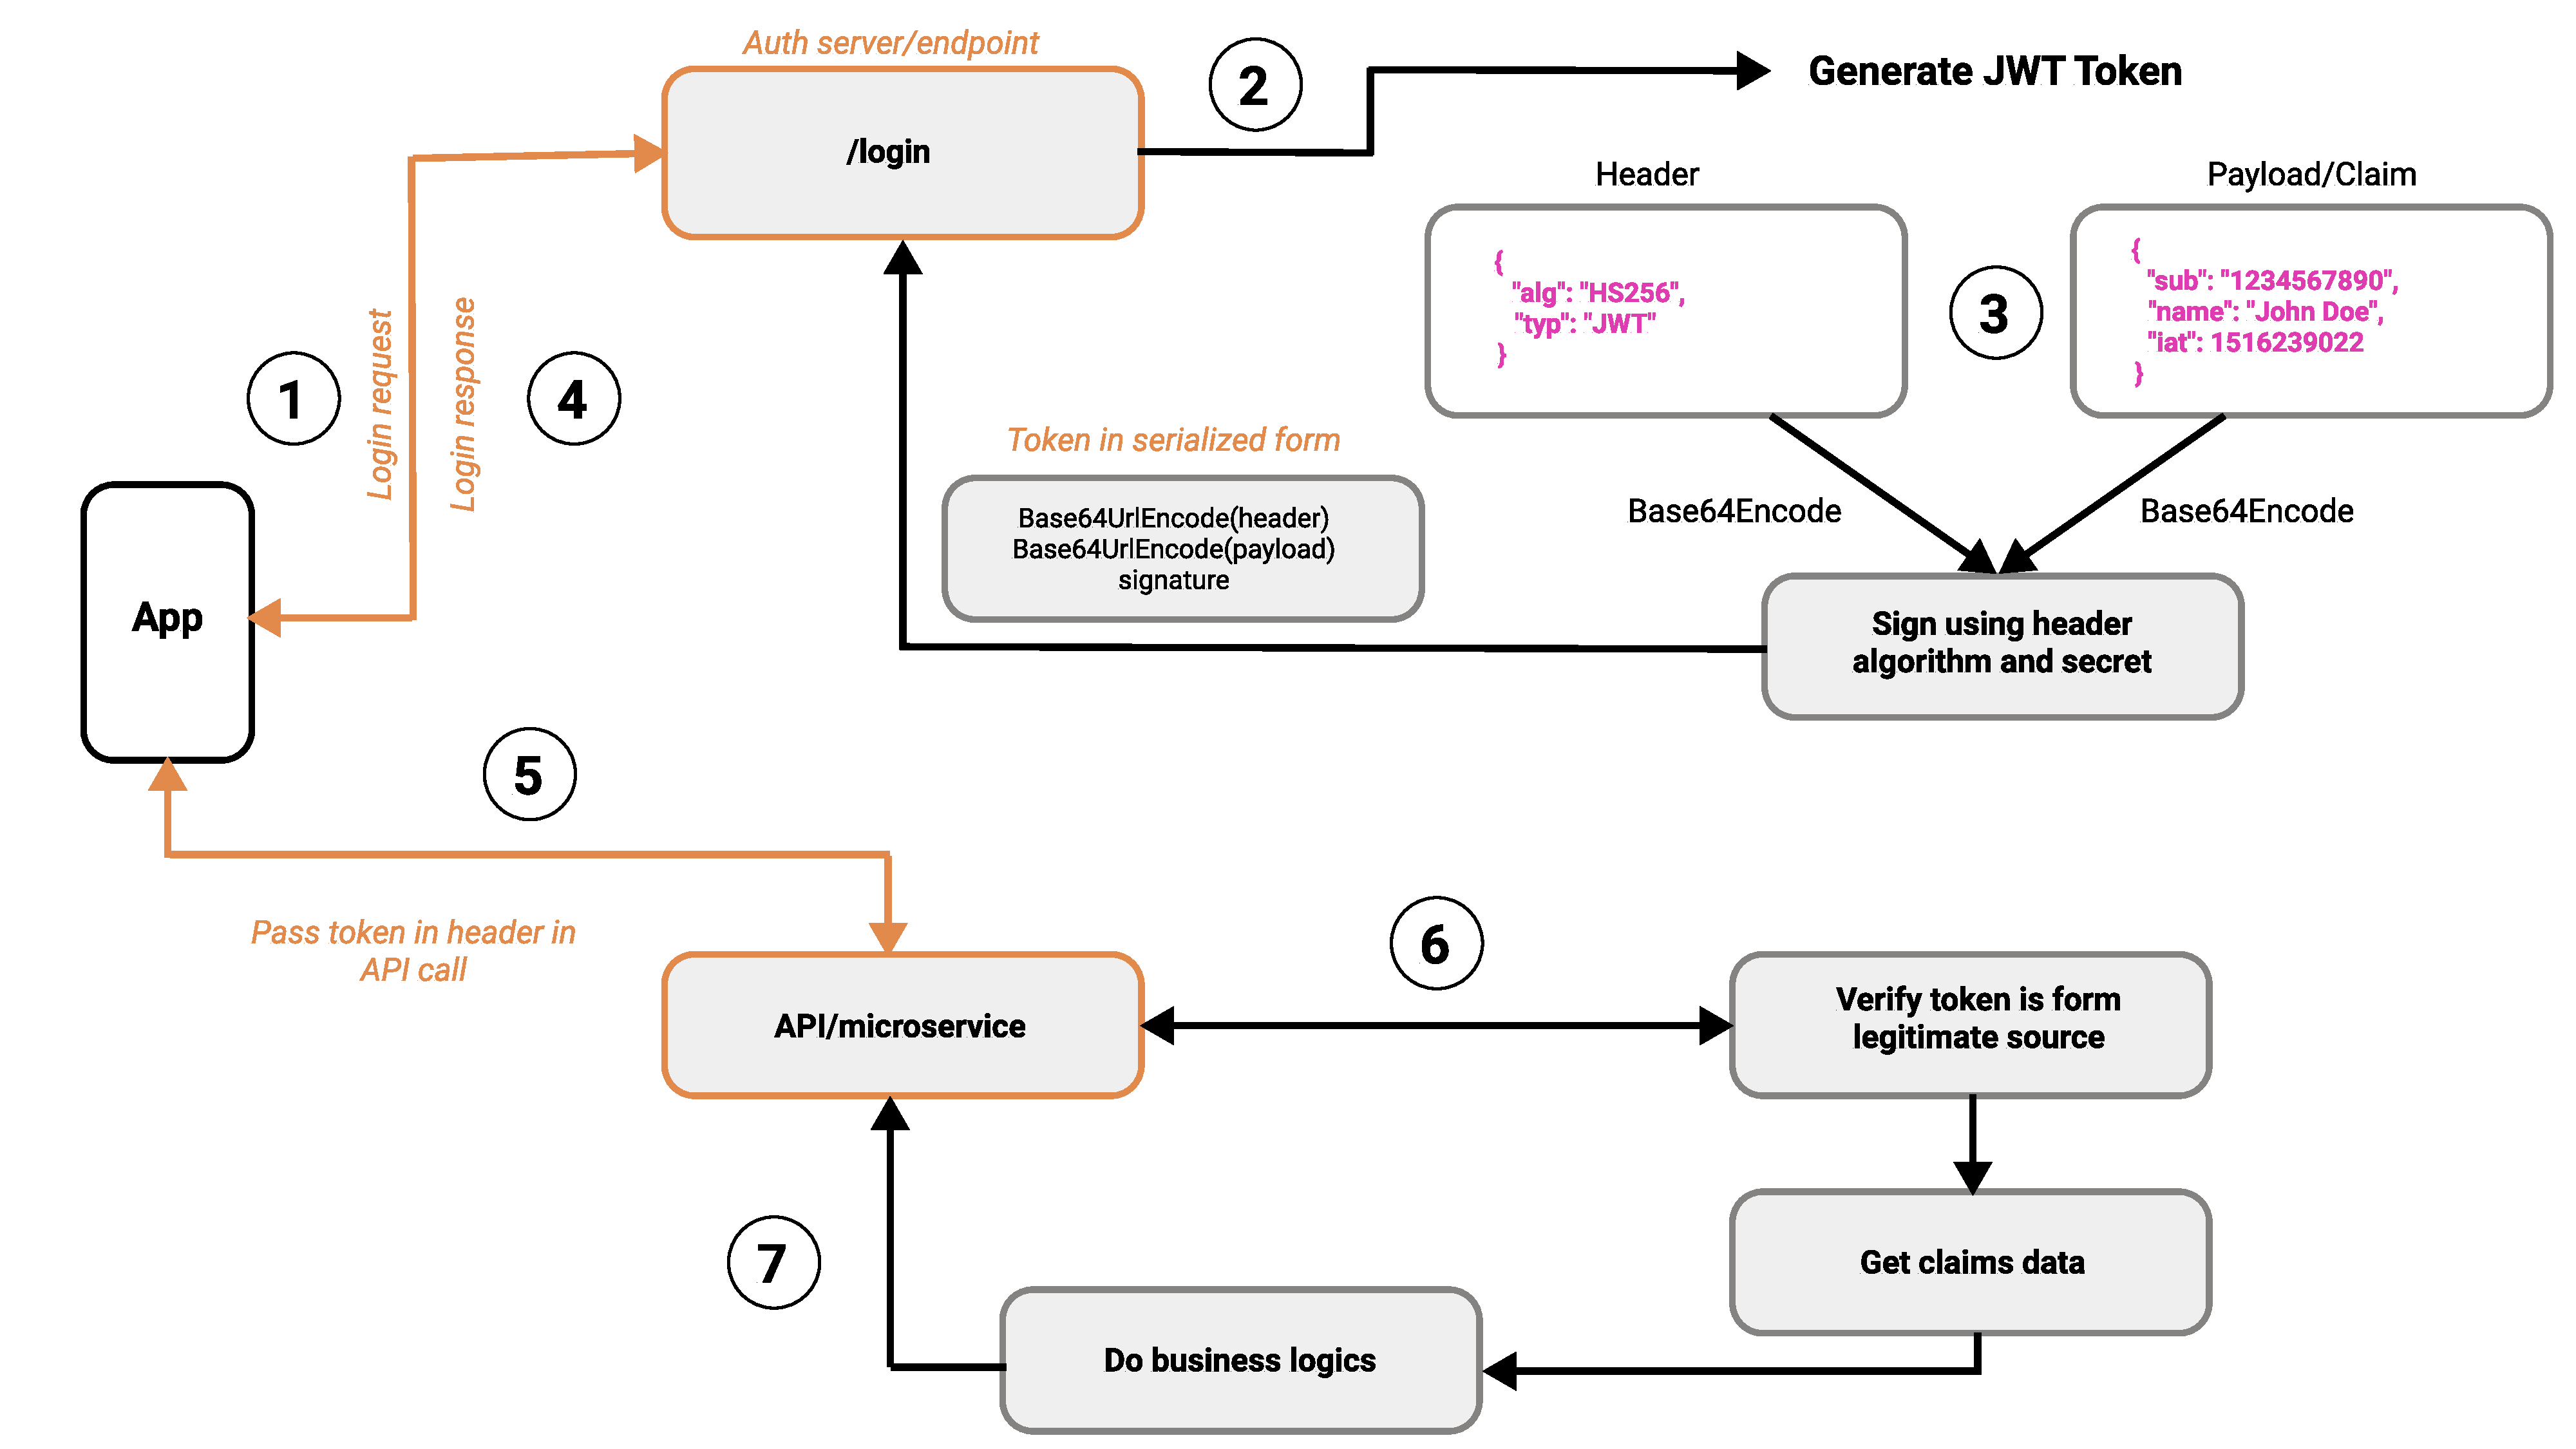
\includegraphics[width=1\textwidth]{Pictures/jwt_auth_scheme.pdf}
    \caption{JWT Authentication principle diagram.}\label{fig:figure3}
\end{figure}

Also, it is worth to add a few basic rules about JWT usage [\cite{RDegges}]
\begin{itemize}
    \item JWT should have a short lifetime, since it cannot be revoked.
    \item JWT should be used in a single time, e.g JWT per request.
\end{itemize}